%%%%%%%%%%%%%%%%%%%%%%%%%%%%%%%%%%%%%%%%
% Class options                        %
%%%%%%%%%%%%%%%%%%%%%%%%%%%%%%%%%%%%%%%%
% Orientation:                         %
% portrait (default), landscape        %
%                                      %
% Paper size:                          %
% a0paper (default), a1paper, a2paper, %
% a3paper, a4paper, a5paper, a6paper   %
%                                      %
% Language:                            %
% english (default), norsk             %
%%%%%%%%%%%%%%%%%%%%%%%%%%%%%%%%%%%%%%%%
\documentclass{psuposter}


\usepackage{natbib}
\usepackage{lipsum}                                % Dummy text
\usepackage[figwidth = 0.98\linewidth]{todonotes}  % Dummy image (and more!)
\usepackage[absolute, overlay]{textpos}            % Figure placement
%\usepackage{hyperref}
\setlength{\TPHorizModule}{\paperwidth}
\setlength{\TPVertModule}{\paperheight}

\setcitestyle{numbers,square}


\title{Scattering Amplitudes and Positive Geometry at Infinity}
\author
{\href{http://www.ias.edu/scholars/arkani-hamed}{Nima Arkani-Hamed}\inst{1}}
%% Optional:
\institute
{
    \inst{1} Institute for Advanced Study, School of Natural Sciences
}
% Or:
%\institute{Contact information}


%% Remove footline:
%\setbeamertemplate{footline}{}


\begin{document}
\begin{frame}
\begin{columns}[onlytextwidth]


\begin{column}{0.45\textwidth - 1cm}
    \begin{block}{Speaker Biographic Summary}
    	\begin{center}
	    	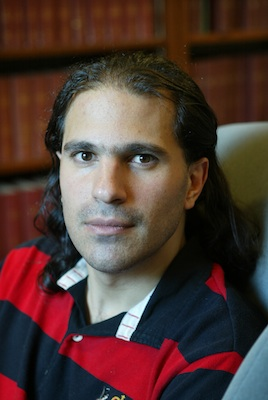
\includegraphics[width=0.6\textwidth]{psuposter-images/arkani-hamed}    		
    	\end{center}
    	Nima Arkani-Hamed is a theorist, based at the Institute of Advanced Studies, with wide-ranging interests in fundamental physics.  He is concerned with the relation between theory and experiment, with a special focus on current and future particle accelerators as well as cosmological observations. His research has shown how the extreme weakness of gravity, relative to other forces of nature, might be explained by the existence of extra dimensions of space, and how the structure of comparatively low-energy physics is constrained within the context of string theory. 
For his seminal contributions to outstanding problems in particle physics, novel realizations of supersymmetry, theories for dark matter, and the exploration of new mathematical structures in gauge theory scattering amplitudes, Prof. Arkani-Hamed was awarded the Fundamental Breakthrough in Physics prize in 2012 \cite{NimaArkaniHamed}. 
%        This paragraph represents the speaker bio. Include their name, affiliation (yes it is included above too..). Also describe their educational background briefly, as well as research interests. If they have won any notable awards / etc, try to mention that as well.
    \end{block}
%
%    \begin{exampleblock}{Does it come in black?}
%        Sure, use an \textbf{exampleblock}!
%    \end{exampleblock}
%
%    \begin{alertblock}{How do you make it pop?}
%        Use an \alert{alertblock}!
%    \end{alertblock}
%
%    \begin{block}{Method}
%        \lipsum[1]
%    \end{block}

    \begin{block}{Research Interests}
        Nima Arkani-Hamed has contributed to many fundamental fields of physics, including high energy theory, quantum field theory, string theory, cosmology, and collider physics.
        \begin{center}
	    	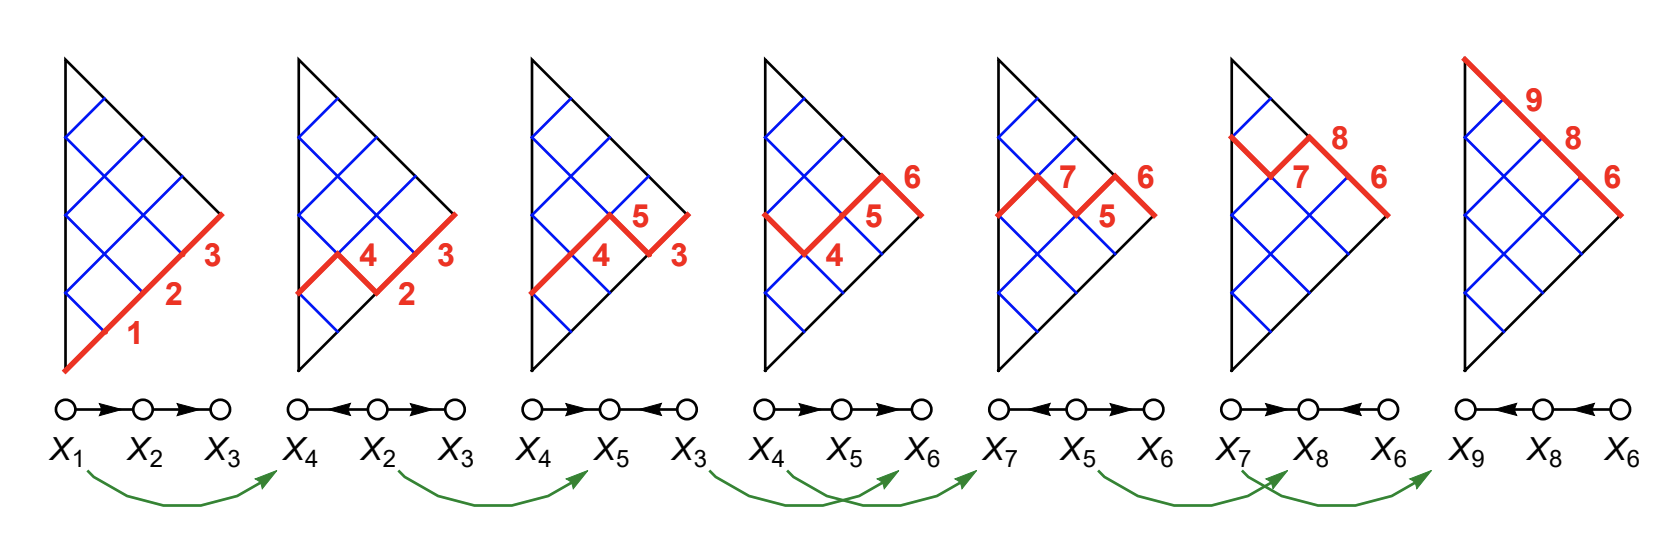
\includegraphics[width=0.98\textwidth]{psuposter-images/quiver-nolabel}    		
    	\end{center}
    	\textit{Above: time evolution of $(1+1)$-dimensional spacetime \cite{arkani-hamedCausalDiamondsCluster2020}}.
    \end{block}
\end{column}


\begin{column}{0.55\textwidth - 1cm}
    \begin{block}{Talk Abstract}
        Elementary particle scattering is perhaps the most basic physical process in Nature. The data specifying the scattering process defines a "kinematic space", associated with the propagation of particles out to infinity. By contrast the textbook approach to computing scattering amplitudes using Feynman diagrams, invokes auxiliary structures beyond this kinematic space--local interactions in the interior of spacetime, and unitary evolution in Hilbert space. This description makes space-time locality and quantum-mechanical unitarity manifest, but hides extraordinary simplicity and infinite hidden symmetries of the amplitude that have been uncovered over the past thirty years. The past decade has seen the emergence of a new picture, where scattering amplitudes are seen as the answer to an entirely different sort of question involving  the notion of "positive geometries" directly in the kinematic space, with surprising and deep connections to a number of contemporary areas of research in mathematics. In this talk I will describe these ideas in a number of examples of direct relevance to real-world physics, where we can see, quite concretely, how the usual rules of space-time and quantum mechanics can arise, joined at the hip, from fundamentally geometric and combinatorial origins
    \end{block}

    \begin{block}{Brief Background}
        Scattering amplitudes are observables measured at the boundary of flat spacetime. They are determined solely by the data of “kinematic space”, corresponding to various ways of labelling the on-shell data of the scattering process. It is thus natural to ask: is there a question, directly posed in this kinematical space, whose answer yields the scattering amplitude, without invoking local evolution through the bulk of spacetime? \cite{arkani-hamedCausalDiamondsCluster2020}
        \begin{center}
	    	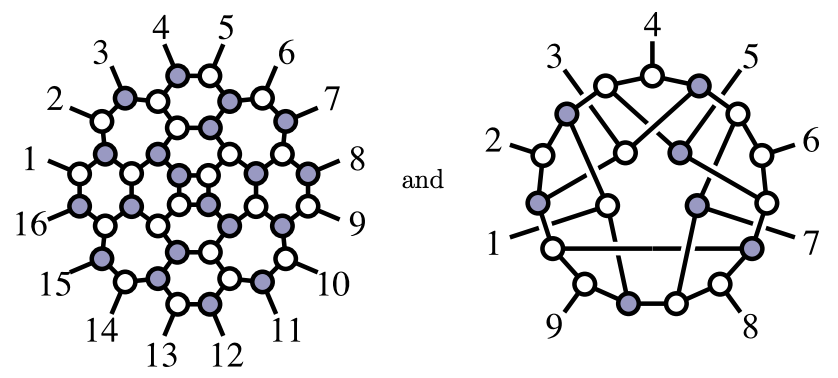
\includegraphics[width=0.6\textwidth]{psuposter-images/on-shell}    		
    	\end{center}
%        $$\lambda_1 \tilde{\lambda}_1 + \lambda_2 \tilde{\lambda}_2 + \lambda_3 \tilde{\lambda}_3 = 0 \iff \left\{ \begin{split}
%        		(A): & \lambda_1 \propto \lambda_2 \propto \lambda_3 \\
%        		(B): & \tilde{\lambda}_1 \propto \tilde{\lambda}_2 \propto \tilde{\lambda}_3 \\
%	        \end{split} \right\}$$
%        \lipsum[3]
		Note that on-shell diagrams such as those above are not Feynman diagrams. There are no “virtual” or “off-shell” internal particles involved: all the lines in these pictures are on-shell (null momenta).  
%		Other terms to mention: helicity [projection of spin onto linear momentum, relation to little group], at-infinity [projective geometry basics, adding ``points at infinity" in projective spaces].
		In this context, ``at infinity" refers to the projective-geometry concept of adding ``points at infinity" where parallel lines, or one-dimensional projective subspaces, intersect.
        \cite{naberTopologyGeometryGauge2011b}
    \end{block}

    \begin{block}{References}
%        \lipsum[1]
        \bibliographystyle{aipnum4-1}
		\bibliography{references}
    \end{block}

%    \begin{block}{Contact information}
%        \lipsum[75]
%    \end{block}
\end{column}


\end{columns}


\begin{textblock}{0.5}(0.18, 0.94)
    \color{white}
    \sffamily
    \textbf{Eberly College of Science}
    \\
    Department of Physics
    
\end{textblock}


\end{frame}
\end{document}